\subsection{Prioritising Explanations}

While the extraction of Minimal CXps provides a set of valid corrections,
it often produces multiple candidates.
For the rejected word $w=\texttt{))))}$,
%
we identified two minimal sets: 
$\text{CXp}_1=\{1,2\}$ (suggesting $\texttt{(())}$) 
and 
$\text{CXp}_2=\{1,3\}$ (suggesting $\texttt{()()}$).

A ranking approach is \textit{Feature Attribution},
which counts the frequency of an index across
all minimal explanations.
%
In our case:
\begin{itemize}
    \item \textbf{Index 1:} Frequency 1.0.
    \item \textbf{Index 2:} Frequency 0.5.
    \item \textbf{Indix 3:} Frequency 0.5.
\end{itemize}

However, symbolic frequency ignores
how likely is resulting correction.
%
In domains like programming, certain structures
(e.g., deeply nested brackets vs. sequential pairs)
have different probabilities.
%
To refine our suggestions, we use
\textbf{Probabilistic Context-Free Grammars (PCFGs)}\cite{pcfg}.

\begin{example}[Rule Counting]
Consider a training dataset
$D=\{\texttt{()()()},\texttt{(())()},\texttt{()(())}\}$.
%
\autoref{fig:trees_dataset} shows the derivation trees,
%
and \autoref{tab:table_counting} the rule counting
to estimate the probability of each production rule
%
($B$ denotes the non-terminal \textit{Balanced}).

\begin{figure}
\centering
    \begin{minipage}[c]{0.3\linewidth}
        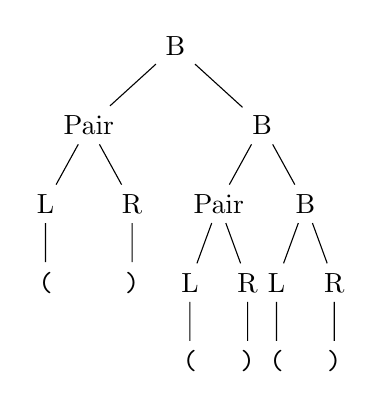
\begin{tikzpicture}[
    level distance=10mm,
    level/.style={sibling distance=22mm/#1}]
  \node {B}
    child { 
        node {Pair}
        child {
            node {L}
            child {node {\texttt{(}}}
            }
        child {
            node {R}
            child {node {\texttt{)}}}
            }
        }
    child { 
        node {B}
        child {
            node {Pair}
            child {
                node {L}
                child {node {\texttt{(}}}
                }
            child {
                node {R}
                child {node {\texttt{)}}}
                }
            }
        child {
            node {B}
            child {
                node {L}
                child {node {\texttt{(}}}
                }
            child {
                node {R}
                child {node {\texttt{)}}}
                }
            }
        };
\end{tikzpicture}
    \end{minipage}
\hfill
    \begin{minipage}[c]{0.3\linewidth}
        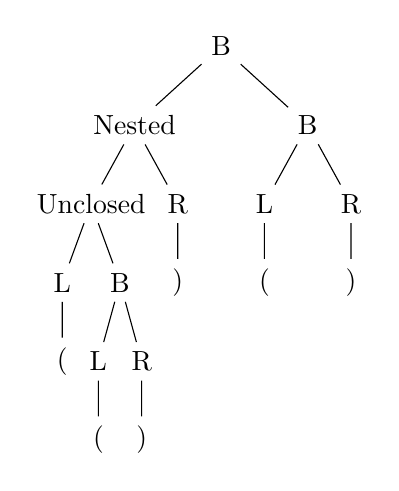
\begin{tikzpicture}[
    level distance=10mm,
    level/.style={sibling distance=22mm/#1}]
  \node {B}
    child {node {Nested}
      child {node {Unclosed}
        child {node {L} child {node {(}}}
        child {node {B} child {node {L} child {node {(}}} child {node {R} child {node {)}}} }
      }
      child {node {R} child {node {)}}}
    }
    child {node {B}
      child {node {L} child {node {(}}}
      child {node {R} child {node {)}}}
    };
\end{tikzpicture}
    \end{minipage}%
\hfill
    \begin{minipage}[c]{0.3\linewidth}
        \input{Figures/PDA/lrllrr.tex}
    \end{minipage}%
\caption{Parse trees for words
\texttt{()()()}, \texttt{(())()}, \texttt{()(())}.}
\end{figure}

\begin{table}[h]
\centering
\renewcommand{\arraystretch}{1.2}
\begin{tabular}{lcc}
\hline
\textbf{Rule} & \textbf{Count} & \textbf{Probability ($P$)} \\ \hline
$B \to L \ R$              & 4 & $4/9 = 44.\overline{4}$ \\
$B \to \text{Pair } B$     & 3 & $3/9 = 33.\overline{3}$ \\
$B \to \text{Nested } B$   & 1 & $1/9 = 11.\overline{1}$ \\
$B \to \text{Unclosed } R$ & 1 & $1/9 = 11.\overline{1}$ \\ \hline
\end{tabular}
\caption{Probability distribution derived from $D$.}
\label{tab:table_counting}
\end{table}

\end{example}

\subsubsection{Ranking Explanations via PCFGs}

To select the best correction, we calculate the probability
of generating suggested correction given a
fixed length constraint.
%
For our running example to explain the rejected word
$w = \texttt{))))}$ we consider the set of all valid
words in the language of length 4
$L_4 = \{ \texttt{()()}, \texttt{(())} \}$.

The total probability for valid words of length 4 is:
\begin{equation}
    P(L_4) = P(\texttt{()()}) + P(\texttt{(())})
\end{equation}

\begin{figure}[t]
\centering
    \begin{minipage}[c]{0.45\linewidth}
        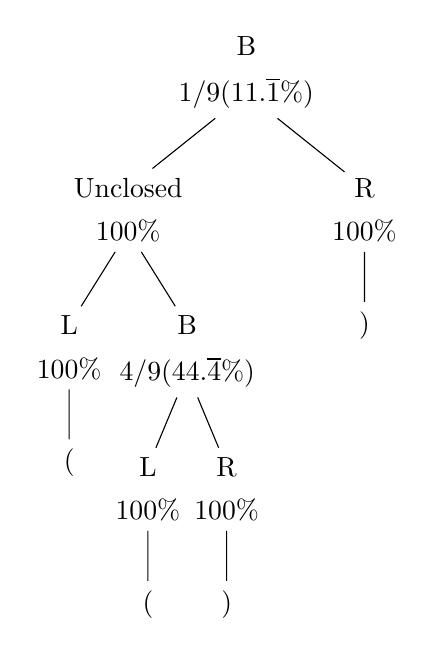
\begin{tikzpicture}[
    level distance=12mm,
    level/.style={sibling distance=30mm/#1}
]
  \node {B}
    % This node is placed at the very start of the children's paths
    node[below=8pt] {$1/9 (11.\overline{1}\%)$}
    child {node {Unclosed}
       node[below=8pt] {{$100\%$} }
      child {node {L} node[below=8pt] {{$100\%$} } child {node {(}}}
      child {node {B}
        node[below=8pt] {{$4/9 (44.\overline{4}\%)$} }
        child {node {L} node[below=8pt] {{$100\%$} } child {node {(}}}
        child {node {R} node[below=8pt] {{$100\%$} } child {node {)}}}
      }
    }
    child {node {R} node[below=8pt] {{$100\%$} } child {node {)}}};
\end{tikzpicture}
    \end{minipage}
    \hfill
    \begin{minipage}[c]{0.45\linewidth}
        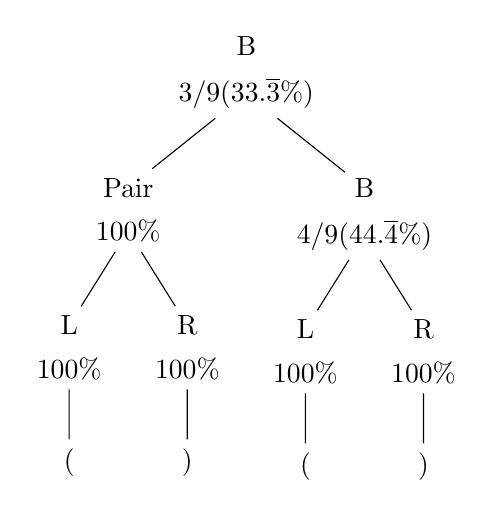
\begin{tikzpicture}[
    level distance=12mm,
    level/.style={sibling distance=30mm/#1}
]
  \node {B}
    % This node is placed at the very start of the children's paths
    node[below=8pt] {$3/9 (33.\overline{3}\%)$}
    child {node {Pair}
       node[below=8pt] {{$100\%$} }
      child {node {L} node[below=8pt] {{$100\%$} } child {node {(}}}
      child {node {R} node[below=8pt] {{$100\%$} } child {node {)}}}
    }
    child {node {B}
       node[below=8pt] {{$4/9 (44.\overline{4}\%)$} }
      child {node {L} node[below=8pt] {{$100\%$} } child {node {(}}}
      child {node {R} node[below=8pt] {{$100\%$} } child {node {)}}}
    };
\end{tikzpicture}
    \end{minipage}
\caption{Parse trees for words
\texttt{(())} and \texttt{()()}.}
\label{fig:trees_dataset}
\end{figure}

Using the estimated rule probabilities,
we compute the likelihood of the corrections
suggested by our CXps (shown in \autoref{fig:trees_dataset}):
\begin{itemize}
    \item $\text{CXp}_1 \to \texttt{(())}$:
    $P(\texttt{(())}) = \frac{1}{9} \times \frac{4}{9} \approx 0.049$
    %
    \item $\text{CXp}_2 \to \texttt{()()}$:
    $P(\texttt{()()}) = \frac{3}{9} \times \frac{4}{9} \approx 0.148$
\end{itemize}

We define the \textit{Relative Likelihood Score} for
a CXp suggesting correction $w'$ as:
%
\begin{equation}
    Score(w')=P(w') / P(L_{|w|})
\end{equation}
%
\begin{equation*}
    Score(\text{CXp}_1)= \frac{0.049}{0.148 + 0.049}\approx \mathbf{0.25} \quad \text{vs} \quad Score(\text{CXp}_2) \approx \mathbf{0.75} 
\end{equation*}
%
Under this PCFG, the correction \texttt{()()}
(suggested by $\text{CXp}_2$)
is more likely than \texttt{(())}
(suggested by $\text{CXp}_1$).
%
This allows the explainer to prioritise
the most statistically probable fix.

\section{Conclusion}

We present a polynomial-time algorithm for
extracting Abductive and Contrastive Explanations
relying on linear calls to a CYK based algorithm.
%
Additionally, incorporating training data,
this approach can prioritise the most relevant
contrastive explanations.
%
Future work will focus on benchmarks
to evaluate the scalability
and a proposal to understand how
can we prioritise abductive explanations.
